\DailyTitle{6274 Log (October 6, 2010)}

\DailySection{Goals}

\begin{enumerate}
\item Read and understand the double spike algorithm
\item Make sure if anyone is doing the vecbos PDMu dataset
\item Make a set of loose cuts to remove obvious noise, and skim through pulse shapes of the rest
\item Port the HCAL ideal pulse shape (as in \texttt{CMSSW}) to \texttt{RooFit}
\item Make a simple timetable for documenting candle analysis
\end{enumerate}

\DailySection{Summary List}

\begin{enumerate}
\item Script to do JES uncertainty fits
\item Ideal hcal pulse shape ported to \texttt{RooFit}
\end{enumerate}

\DailySection{Setting up scripts to fit for JES uncertainty}

Copied the fitting script from two days ago, and applied five times for both calo jet and PF jet.
The script is done so once data come, I can just press button and it will do the fitting.
For current data ($2.66 pb^{-1}$), the result is shown in figures \ref{Figure_6274CaloJet30_JES}
and \ref{Figure_6274PFJet20_JES}.  The correction uncertainties are assumed to be

\begin{enumerate}
\item 10\% overall scale for calojet
\item 5\% overall scale for PF jet
\item $2\% \times |\eta|$ for both types of jets.
\end{enumerate}


\begin{figure}
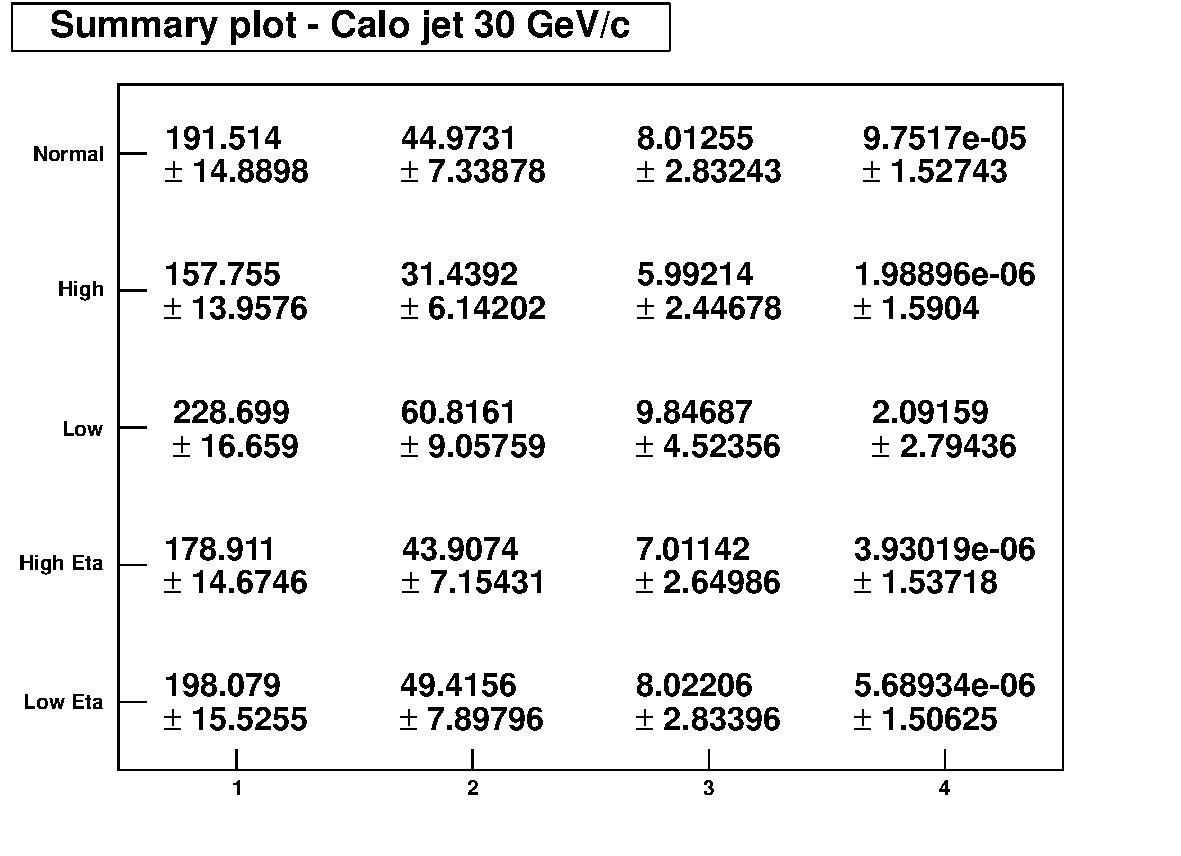
\includegraphics[width=120mm]{DailyLog/6274/6274_CaloJet30_JES}
\caption{Jet energy correction uncertainty estimation for calojet with threshold 30 GeV/c.}
\label{Figure_6274CaloJet30_JES}
\end{figure}

\begin{figure}
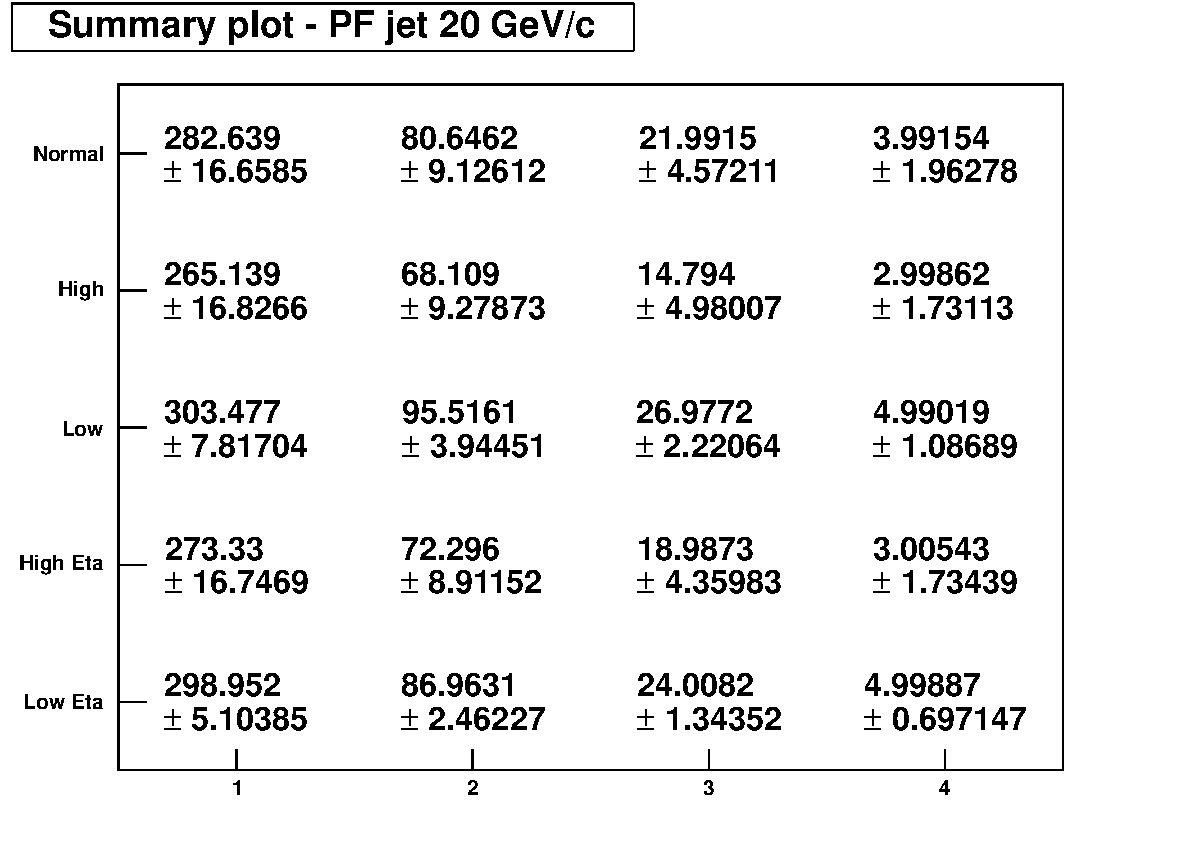
\includegraphics[width=120mm]{DailyLog/6274/6274_PFJet20_JES}
\caption{Jet energy correction uncertainty estimation for particle-flow jet with threshold 20 GeV/c.}
\label{Figure_6274PFJet20_JES}
\end{figure}


\DailySection{Port ideal HCAL pulse shape to \texttt{RooFit} and include in the brainstorming plots}

Copied out the \texttt{HcalPulseShapes.cc} and \texttt{HcalPulseShapes.h} from \texttt{CMSSW382}.
The files are not dependent on root libraries or \texttt{CMSSW}, and I hacked the files to get the ideal shape.
The ported pulse shape is shown in figure \ref{Figure_6274_IdealHcalPulseshape}.

\begin{figure}
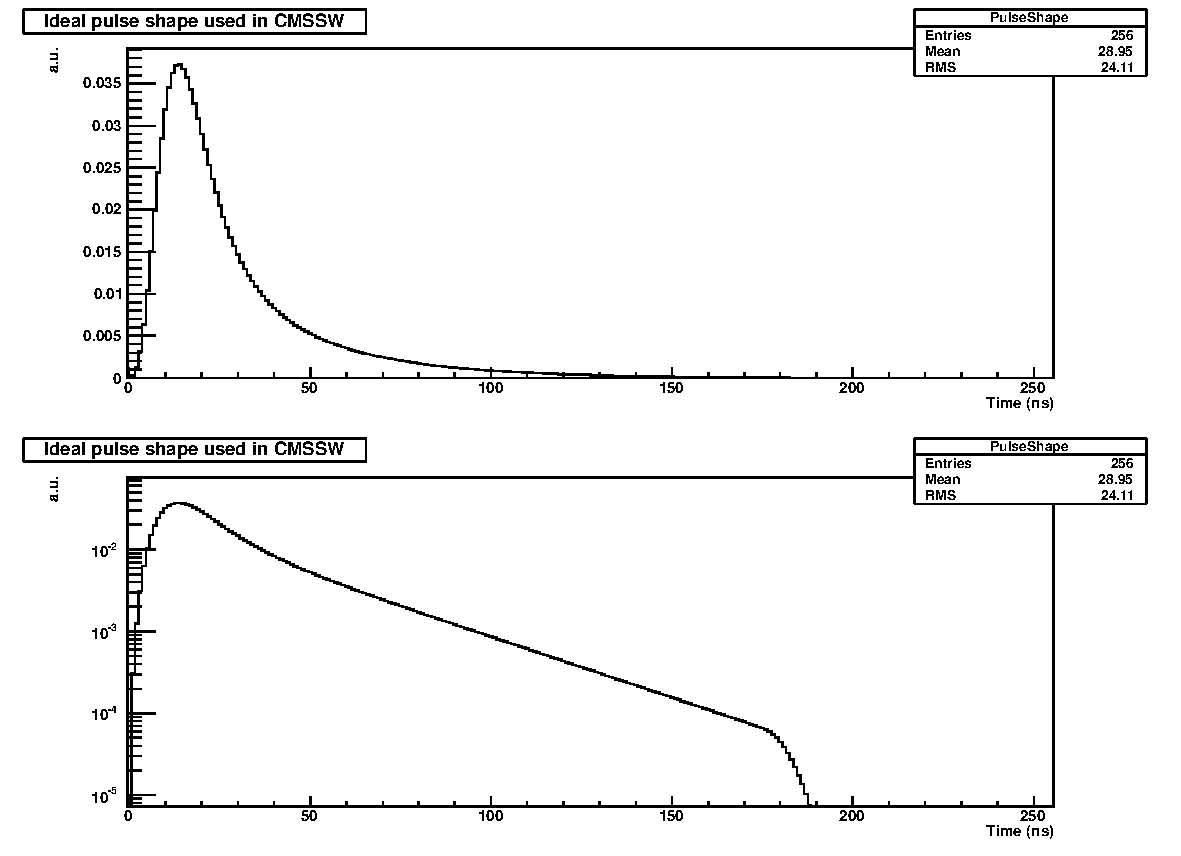
\includegraphics[width=120mm]{DailyLog/6274/6274_IdealHcalPulseshape.pdf}
\caption{Extracted hcal ideal pulse shape from \texttt{CMSSW} version \texttt{3\_8\_2}.  The two panels
are the same histogram, except that one is in log scale.}
\end{figure}

\DailySection{Reflection}

No work is done after going home....not good....

\DailySection{Goals for next work day}

\begin{enumerate}
\item Make a list of things that need to be documented for the ZJet candle analysis
\item Check what Artur needs in terms of vecbos ntuples
\item Try out Hcal DQM test bench on lxplus.
\item Double-spike algorithm.
\end{enumerate}



